\chapter{State}
\label{ch:state}

Pause a machine between two instructions. The arithmetic has stopped, but its
result is only one part of what remains. Registers contain words. Memory
contains bytes. A program counter identifies the next instruction. Condition
bits remember facts that a later branch may use. The machine is either able to
continue, halted, or trapped for a reason.

Leave one of these parts out and two programs may appear to agree only because
we forgot where to look. We will therefore build the complete state first.
For a particular question, we may then state which parts of that state matter.

\begin{archive}[title={\iconArchive\ A stored program needs a place to resume}]
The 1945 EDVAC report divided a proposed computing system into organs for
arithmetic, control, memory, input, and output. Its terminology is historical,
but the design problem remains current: after one operation, the machine must
retain enough information to determine the next. Modern architectural state
is not copied from that report; it is one descendant of the need the report
made explicit.\autocite{vonneumann1945edvac}
\end{archive}

The important word is \emph{enough}. We could describe every charge, latch,
queue entry, and temperature in a physical processor. Such a description
would be too large for our purpose and still incomplete. We could describe
only the destination register. That would be small, but too weak to predict a
branch or a memory access. A state model earns its size by the questions it
can answer.

State is therefore a boundary around relevant history. Once the state is
fixed, the next architectural step should not need a secret account of how
the machine arrived there. Two executions that reach the same A0 state face
the same A0 successors under the same program. Their earlier paths may differ,
but the transition rule receives the same input.

\begin{definition}[title={State sufficiency}]
A state description is sufficient for a transition model when the modeled
next-step possibilities depend only on that state and the declared external
inputs, not on an unrecorded execution history.
\end{definition}

State sufficiency is a modeling requirement, not a physical claim that
history vanishes entirely.
A cache or branch predictor can retain effects of earlier execution. A0 omits
them, so A0 cannot answer a question whose next result depends on those
effects. A timing model may restore them as state. The right snapshot changes
with the promised observation.

\section{The teaching machine}
\label{sec:a0-state}

The abstract machine used in this book is A0. Its word width \(w\) is a
positive multiple of eight. The width-four patterns in Chapter 1 remain useful
on a blackboard, but they are not complete A0 machine states. Full A0 begins at
one byte because its memory is byte-addressed.

\begin{definition}[title={A0 machine state}]
An A0 \keyterm{machine state} is
\[
  S=(R,M,pc,Z,N,C,V,O).
\]
The map \(R\) assigns a \(w\)-bit word to each of the eight registers
\(r_0,\ldots,r_7\). The finite map \(M\) assigns bytes to valid data
addresses. The \(w\)-bit word \(pc\) is the program counter. The bits
\(Z,N,C,V\) record zero, negative, carry, and overflow conditions. The outcome
\(O\) is running, halted, or trapped with a reason.
\end{definition}

\begin{figure}[htbp]
\centering
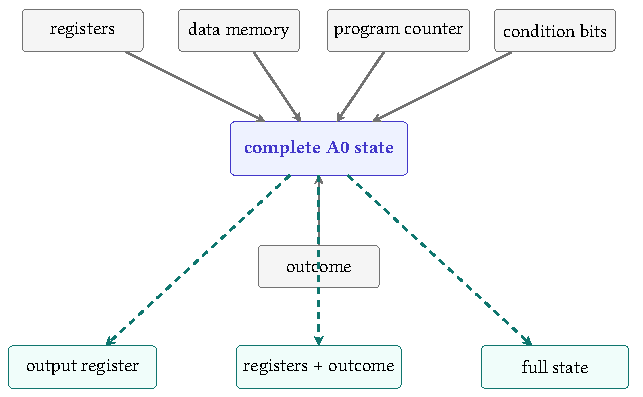
\includegraphics[width=0.94\textwidth]{figures/a0-state-inventory}
\caption{A0 gathers every modeled component into one complete state. An
observation projects that state to the information a claim exposes.}
\figalt{Registers, memory, program counter, condition bits, and outcome enter A0 state, which projects to three observations.}
\label{fig:a0-state-inventory}
\end{figure}

The tuple is not a bag of unrelated fields. Its components constrain one
another through instruction rules. A running state permits a step; a halted or
trapped state does not. The program counter supplies the next fetch address.
Register contents may supply operands or addresses. Condition bits may supply
a branch predicate. Memory supplies bytes only at addresses in its finite
domain. Chapter 3 will define the transformations that preserve these
connections.

Object \obj{A0.def.state} records this contract. Every register is ordinary:
A0 has no hardwired zero register and no implicit stack pointer. The condition
bits are named state, not comments about the previous line. If an instruction
writes one of them, a later instruction can observe that write.

Program code is not part of \(M\). An A0 program supplies a separate, finite
map of immutable instruction bytes and an entry address. This choice rules out
self-modifying code in the first model. It also prevents a data store from
silently changing the next instruction. Chapter 5 will add the program to the
execution setting; for now we are describing the snapshot on which one step
acts.

Separating code from data is a modeling decision, not a claim about all real
machines. It gives the first A0 model a stable program while we learn to reason
about data memory. A theorem under this separation says nothing about
self-modifying programs unless a later model adds code memory to the writable
state and repairs every affected definition.

The outcome needs three cases. A running state may take a step. A halted state
has finished by executing \code{halt}. A trapped state records that execution
could not continue under an A0 rule, such as an invalid memory range. Halt and
trap both have no successor, but they do not mean the same thing. A program
that finishes and a program that fails are not interchangeable merely because
both stop.

\begin{example}[title={Three stopped descriptions}]
Suppose the last destination contains 42 in three states. In the first, the
outcome is halted. In the second, an invalid load has trapped. In the third,
the outcome remains running but no further step has been requested. Looking at
the destination alone collapses three different execution situations into one
number. A claim about successful completion must include the outcome.
\end{example}

The reason attached to a trap also matters when a claim distinguishes failure
modes. A0 will name reasons such as illegal encoding, incomplete fetch, and
invalid data range. We may later choose an observation that retains only the
fact of trapping, but the complete state does not discard the reason first.

\subsection{Well-formed states and componentwise equality}

Not every tuple of mathematical objects is an A0 state. The width must be a
positive multiple of eight. Each register value and the program counter must
fit that width. Every memory value must be a byte, and every memory key must be
a width-\(w\) address. Condition fields are bits. The outcome must be one of the
declared cases, with a recognized reason when it is trapped.

A constructor should enforce these requirements once. Later instruction
rules can then assume they receive a well-formed state and must return another
one. Without that invariant, every transition theorem carries distracting
side cases about a nine-bit value in an eight-bit register or a memory entry
that is not a byte.

Two A0 states are equal exactly when their corresponding components are equal:
the same register map, memory map, program counter, four conditions, and
outcome. This componentwise rule gives both proof directions. To establish
state equality, establish every component. To refute it, one unequal component
is enough.

\begin{figure}[htbp]
\centering
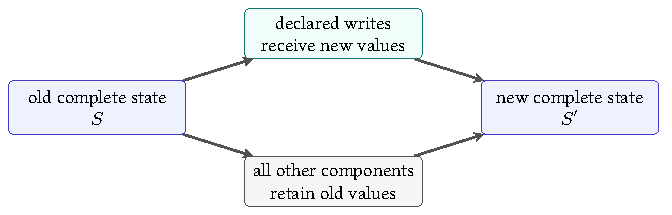
\includegraphics[width=0.82\textwidth]{figures/state-transition-frame}
\caption{A complete transition combines declared new values with a frame
condition that preserves every component outside the write set.}
\figalt{An old complete state splits into changed components and preserved components, which join into the new complete state.}
\label{fig:state-transition-frame}
\end{figure}

The preservation branch in Figure~\ref{fig:state-transition-frame} is a
\keyterm{frame condition}. It says what the instruction leaves alone. A state
diff is a convenient way to display the other branch, but a diff is complete
only when it is interpreted against an old state and a rule that preserves
everything omitted from it.

A destination-only test is therefore weak. It checks one changed component
without checking conditions, control, memory, outcome, or the frame. A
complete-state checker can still print a compact diff for the reader. It must
derive that diff from states whose equality and preservation it actually
checks.
Compact presentation and complete checking can therefore coexist without
weakening the state contract.

\section{Which state belongs to the architecture?}

The tuple above is an \keyterm{architectural state}: it contains the parts
that A0 instructions are defined to read or change. A physical processor
needs much more. It may contain pipeline registers, cache tags, branch
predictor entries, queues, and circuitry that has no name in an assembly
program.

Whether those parts belong in a model depends on the question. If the question
is whether two additions leave the same A0 state, cache replacement policy is
irrelevant because A0 has no cache state. If the question is how long the two
additions take on a particular processor, the A0 tuple is insufficient. A
smaller model is not false merely because it omits timing; it is false when it
is used to answer a timing question.

One practical test sharpens the word \emph{architectural}. Ask whether the
declared instruction semantics can read the component, write it, or expose it
through a modeled outcome. If yes, the component belongs in the state for that
semantic question. If it affects only how a particular implementation reaches
the result, it may remain outside a functional model. The answer can change
when the question changes: cache contents are outside A0 functional
equivalence and inside many timing or leakage models.

\begin{warning}[title={An omitted component is a theorem premise}]
Every omitted kind of state limits the claims that follow. Leaving caches out
does not assert that caches do not exist. It asserts that the present
observation and transition rules do not speak about their effects.
\end{warning}

The distinction cuts both ways. Different internal executions may have the
same architectural result. The processor is free to use either route if its
contract permits both. Yet equal values in one destination register need not
mean equal architectural results. Memory, flags, the program counter, and the
outcome can still differ.

Consider two paused A0 states. Both have 7 in \(r_0\), 12 in \(r_1\), the same
memory, and a running outcome. In the first state \(pc=8\); in the second
\(pc=12\). If we record only \(r_0\), the difference disappears. At the next
step it may decide which instruction executes. The missing component was not
minor. It was merely unobserved.

State completeness is therefore relative to a declared machine contract. The
A0 tuple is complete for A0 because every A0 instruction effect must appear in
that tuple or its outcome. It is not complete for RV64, x86-64, or a physical
processor merely because it is written with eight fields. Each later slice
must perform its own inventory.

\section{What we choose to observe}
\label{sec:state-observation}

Now consider a less severe difference. Program \(p\) leaves 7 in \(r_0\) and
19 in scratch register \(r_3\). Program \(q\) also leaves 7 in \(r_0\), but
leaves 20 in \(r_3\). A caller that receives only \(r_0\) may be unable to
tell. A comparison of all registers can tell at once.

\begin{definition}[title={Observation}]
An \keyterm{observation} is a declared function from a complete state to the
information exposed by a claim. Two states agree under observation \(A\) when
\[
  A(S_1)=A(S_2).
\]
\end{definition}

Object \obj{A0.def.observation} fixes this role. An observation may select one
register, all registers, a range of memory, the outcome, or a declared
combination. The complete state still exists. The observation says which
differences the claim exposes.

Figure~\ref{fig:a0-state-inventory} shows three observations, ordered from
narrow to broad. This ordering is not always a straight line. One observation
might expose a memory range and hide all registers; another might expose two
registers and no memory. Neither necessarily contains the other. The useful
relation is whether one observation can be derived from another. If it can,
the first reveals no distinction that the second has already forgotten.

\begin{figure}[htbp]
\centering
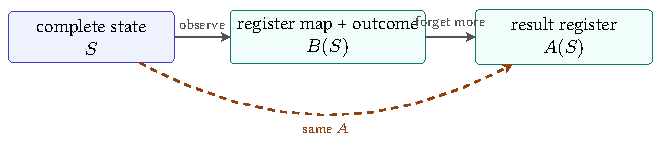
\includegraphics[width=0.78\textwidth]{figures/observation-factorization}
\caption{A narrower observation can factor through a broader one. Once the
broader result is known, an additional projection obtains the narrower result
without consulting the complete state again.}
\figalt{A complete state maps to registers and outcome, which maps to the result register; a dashed direct arrow gives the same result observation.}
\label{fig:observation-factorization}
\end{figure}

In the diagram, \(A=f\mathbin{\circ}B\) for a function \(f\) that selects the
result register. Agreement under \(B\) then implies agreement under \(A\):
equal broad observations remain equal after applying \(f\). The reverse may
fail because \(f\) discards the other registers and the outcome.

An observation partitions the state space into groups that it cannot
distinguish. Every state with the same observed result belongs to the same
group, even if hidden components differ. A broader observation usually splits
some of those groups. Full-state observation leaves only groups of equal
states.

The partition view explains why an observation is neither correct nor
incorrect by
itself. It is adequate or inadequate for a context. If a caller can read only
the result register and outcome, grouping states that differ solely in a dead
scratch register may be appropriate. If a later branch reads a condition bit,
an observation that groups different condition values is too coarse for
replacement before that branch.

\begin{keyidea}[title={Observation fixes what counts as a difference}]
Choose the observation from the contract of the surrounding context. Then ask
whether the programs agree under it. Choosing the projection after seeing a
counterexample changes the question instead of answering it.
\end{keyidea}

The scratch-register example gives a small proof of an important limit. Let
\(A(S)=R[r_0]\). Both final states map to 7, so they agree under \(A\). Let
\(B(S)=R\), the complete register map. The first map sends \(r_3\) to 19 and
the second sends it to 20, so \(B(S_p)\ne B(S_q)\). Agreement after applying
one observation does not imply equality of the underlying states.

The converse direction is safe. If two complete states are equal, every
function maps them to equal observations. Observation can forget a
difference; it cannot create one between equal inputs.

\begin{proofkit}[title={\iconProofKit\ Equality survives every observation}]
Assume \(S_1=S_2\). An observation \(A\) is a function, so replacing an input
by an equal input cannot change its output. Therefore \(A(S_1)=A(S_2)\).
The reverse implication needs more: it holds only when \(A\) is injective on
the states under discussion. A projection to one register is not injective
because many complete states share that register value.
\end{proofkit}

The tiny argument will later carry a large burden. Full-state equivalence
implies agreement under every declared observation. Observational equivalence
does not imply full-state equality unless the observation retains enough
information. When a proof uses the reverse direction, it must establish that
extra premise rather than smuggle it in through the word \emph{equivalent}.

The freedom is useful and dangerous. We must choose the observation as part
of the claim, before seeing which components a proposed rewrite happens to
disturb. Otherwise any difference can be dismissed after the fact by choosing
a function that forgets it. That would not establish equivalence. It would
only tailor the question to the answer.

We also need the observation to be stable across both programs. Comparing
program \(p\) under one observation with program \(q\) under another can make
any two results appear equal by choosing constant functions. One claim uses
one declared observation, applied to both sides.

\begin{tryit}[title={Design the smallest honest observation}]
A routine receives two words, uses \(r_3\) as scratch space, writes its answer
to \(r_0\), and may trap on an invalid input. A caller may later read \(r_0\)
and distinguish normal return from a trap, but it promises not to read
\(r_3\). Write an observation that exposes exactly those facts. Then remove
one component and describe the false replacement it would permit.
\end{tryit}

\begin{example}[title={One result, three questions}]
Suppose two runs finish with the same \(r_0\), different \(C\), and different
outcomes: one halted and one trapped. They agree under the observation
\(A(S)=R[r_0]\). They disagree under an observation of \((R[r_0],C)\), and
they disagree under any observation that includes the outcome. All three
statements are exact. Only the first would be useful to a context that cannot
inspect the carry bit or distinguish success from failure.
\end{example}

\subsection{Initial-state premises restrict the question honestly}

A program theorem rarely concerns every well-formed state. It may require a
running outcome, a particular entry program counter, valid input addresses,
or argument words in selected registers. These facts form the
\keyterm{initial-state premise}. They identify the states from which the claim
promises behavior.

The premise differs from the observation. A premise restricts which inputs
must be considered. An observation selects which output differences count.
Weakening the premise asks the program to handle more starting states.
Broadening the observation asks it to preserve more visible output state.
Both changes make a claim harder, but they act at opposite ends of execution.

\begin{example}[title={One address premise prevents an expected trap}]
Suppose a routine loads four bytes beginning at the address in \(r_1\). A
premise that all four addresses exist removes invalid-range inputs from the
claim. Without that premise, a correct theorem must include trapped outcomes
or establish some other reason the range is valid. Hiding the outcome in the
final observation would not make the load succeed.
\end{example}

Premises must be stated before testing candidate programs. Otherwise a failed
input can be excluded merely because it is inconvenient, just as an output
difference can be hidden by choosing a narrow observation afterward. Later
objects will bind the input premise and output observation beside the program
and machine model so neither can drift during search or replay.

For cross-ISA work, the premise may be relational. It can say that an A0
register and an RV64 register represent the same argument while their unused
registers differ. The output observation then asks whether the related runs
produce corresponding results and outcomes. Equality of the raw state tuples
is neither expected nor required.
What matters is the declared correspondence at entry, at matched control
points, and at the observed exit.

\section{State in the two companion machines}
\label{sec:paired-state}

A0 now gives us an inventory to carry to a real instruction set. We ask which
registers exist, what the program counter denotes, which condition state an
instruction can read or write, how memory enters the model, and which
exceptional outcomes the selected instruction forms admit.

For the later RV64 slice, the integer register named \code{x0} needs special
treatment. A model that stores and later returns an arbitrary word from
\code{x0} would describe a different machine. The slice must also name its
program counter, ordinary integer registers, memory assumptions, and relevant
exceptional outcomes.

For the later x86-64 slice, the model must name the selected general-purpose
registers, \code{RIP}, memory, and exactly which \code{RFLAGS} bits matter to
the included forms. An arithmetic replacement that preserves its destination
but changes a later branch condition is not full-state equality. It may be
valid under a narrower observation, but only if the surrounding program is
unable to rely on the omitted flag.

These are state questions, not verdicts about RISC and CISC. One architecture
has a special integer-register rule; the other example carries selected
condition bits. The exact slices and source revisions must be fixed before
either description supports an architectural claim.

The comparison also explains why cross-ISA states will not be equal. A0 has
eight ordinary registers and four named condition bits. RV64 has a larger
integer register file with a special zero-register rule in the planned slice.
The selected x86-64 slice has its own register names, partial-register rules,
and condition state. Later we will relate states by what they represent, not
by demanding identical tuples.

\begin{keyidea}[title={A state relation is not an observation}]
An observation extracts information from one machine state. A state relation
connects states from two possibly different machines. Cross-ISA proofs need
both: a relation for corresponding inputs and intermediate states, and an
observation for the outputs the claim exposes.
\end{keyidea}

\section{The implementation boundary}

We can now say what an executable A0 state package must do. It must construct
the entire tuple, enforce the width and memory conditions, represent all three
outcomes, and apply observations without changing the state they inspect.
Object \obj{OP.a0.state-memory} records that implementation obligation for
Axeyum.

The controls follow from the reader examples. A projection checker must reject
a claim that two unequal full states are equal merely because \(r_0\) matches.
An outcome test must distinguish halt from trap. A state constructor must
reject a width that is not a positive multiple of eight. A memory test must
not allow an address outside the finite map.

The first Axeyum lesson at this layer should remain small. Construct two A0
states that differ only in \(r_3\). Apply an output-register observation and a
full-register observation. The first results should agree; the second should
produce the differing register as a witness. Mutate the projection so that it
silently omits a requested component. The negative control must reject the
mutated route.

The serialized state should be canonical enough for an artifact digest to
bind one meaning. Register order, address order, word width, outcome tags, and
trap reasons must not depend on a hash-map iteration order or a Python display
choice. A reader-facing table may choose a pleasant order, but replay should
parse one explicit representation and reject duplicates, missing fields, and
out-of-width values.

Observation descriptions also belong in the artifact. A label such as
\code{result} is insufficient unless it resolves to a declared register,
width, and outcome policy. The checker should rebuild the observation from
that declaration and apply it to both full states. It should not trust stored
observation outputs that could have been edited independently of their source
states.

The Python layer can make this lesson direct. It constructs states through
the bound Rust types, asks for named observations, and prints both the compact
result and any separating component. Rust owns width checking, canonical
serialization, projection, and comparison. Python owns presentation and the
sequence of questions; it does not carry a second definition of state.

That exercise teaches the division of labor. Executable state constructors
make malformed states hard to express. Observation functions state what the
claim exposes. A solver may search for two states that a proposed implication
handles incorrectly. A replay checks the returned states through the same
executable definitions. None of those layers decides which observation is
appropriate for the surrounding program; that remains part of the theorem we
choose to state.

No such Axeyum package accompanies this draft yet. The tuple and the arguments
in this chapter are definitions and reader reasoning; they are not a hidden
machine-proof route. That boundary will remain visible until the executable
state and its controls exist.

A state is a still picture. It tells us where every modeled value is, what may
happen next, and whether another step is allowed. It does not move itself.
Chapter 3 supplies the object that turns one such picture into the next.

\section{Exercises}

\begin{enumerate}
\item \textbf{Execute.} Write an A0 state of width eight with register
\(r_i=i\), memory bytes \code{10}, \code{20}, \code{30}, \code{40} at
addresses 0 through 3, \(pc=0\), cleared condition bits, and a running
outcome. Evaluate observations that select \(r_0\), all
registers, and \((pc,O)\).
\item \textbf{Break.} Construct two states that agree in every register but
differ in memory. Give an observation that hides the difference and one that
exposes it. Explain why neither observation changes the states.
\item \textbf{Prove.} Show that complete-state equality implies agreement
under every observation. Then use a two-element example to show that the
converse is false for a non-injective observation.
\item \textbf{Transfer.} For a proposed RV64 state and a proposed x86-64
state, list one special component or rule that has no direct A0 counterpart.
State the functional question that makes it relevant.
\item A sequence changes \(C\) but no register or memory byte. State two
replacement claims for which that fact leads to different answers.
\item Give one timing question for which A0 architectural state is too small.
Name the missing physical information without adding it to A0.
\item \textbf{Execute.} Starting from the state in the first exercise, change
only \(pc\), then only \(O\), then one memory byte. For each change, list the
observations in Figure~\ref{fig:a0-state-inventory} that can detect it.
\item \textbf{Prove.} Let observation \(A\) be computable from observation
\(B\). Show that agreement under \(B\) implies agreement under \(A\). Give an
example showing that the reverse implication can fail.
\item \textbf{Break.} Define an observation after inspecting two unequal
states so that it hides their only difference. Explain why the resulting true
equality does not support the original full-state claim.
\item \textbf{Transfer.} Sketch a relation between an A0 input state and a
future real-ISA input state for a routine with two arguments and one result.
Name what the relation deliberately leaves unmatched.
\end{enumerate}
